% Created by tikzDevice version 0.12.3 on 2019-12-17 19:18:25
% !TEX encoding = UTF-8 Unicode
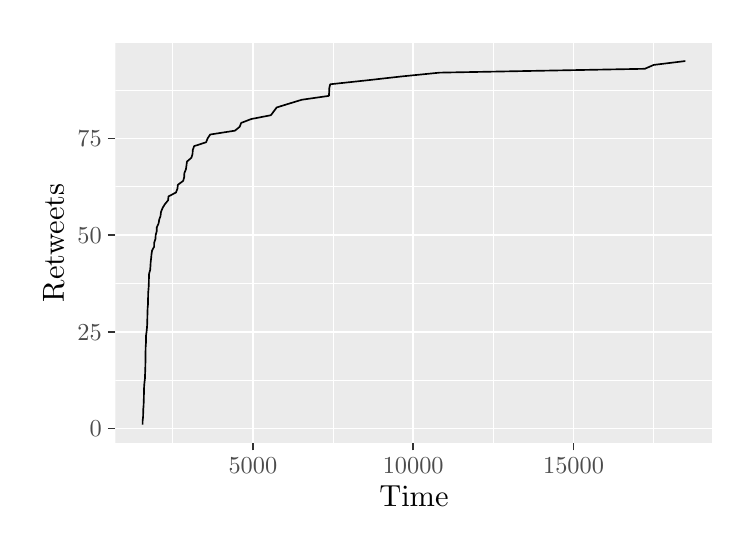
\begin{tikzpicture}[x=1pt,y=1pt]
\definecolor{fillColor}{RGB}{255,255,255}
\path[use as bounding box,fill=fillColor,fill opacity=0.00] (0,0) rectangle (252.94,180.67);
\begin{scope}
\path[clip] (  0.00,  0.00) rectangle (252.94,180.67);
\definecolor{drawColor}{RGB}{255,255,255}
\definecolor{fillColor}{RGB}{255,255,255}

\path[draw=drawColor,line width= 0.6pt,line join=round,line cap=round,fill=fillColor] (  0.00,  0.00) rectangle (252.94,180.68);
\end{scope}
\begin{scope}
\path[clip] ( 31.71, 30.69) rectangle (247.44,175.17);
\definecolor{fillColor}{gray}{0.92}

\path[fill=fillColor] ( 31.71, 30.69) rectangle (247.44,175.17);
\definecolor{drawColor}{RGB}{255,255,255}

\path[draw=drawColor,line width= 0.3pt,line join=round] ( 31.71, 53.32) --
	(247.44, 53.32);

\path[draw=drawColor,line width= 0.3pt,line join=round] ( 31.71, 88.26) --
	(247.44, 88.26);

\path[draw=drawColor,line width= 0.3pt,line join=round] ( 31.71,123.19) --
	(247.44,123.19);

\path[draw=drawColor,line width= 0.3pt,line join=round] ( 31.71,158.13) --
	(247.44,158.13);

\path[draw=drawColor,line width= 0.3pt,line join=round] ( 52.40, 30.69) --
	( 52.40,175.17);

\path[draw=drawColor,line width= 0.3pt,line join=round] (110.35, 30.69) --
	(110.35,175.17);

\path[draw=drawColor,line width= 0.3pt,line join=round] (168.29, 30.69) --
	(168.29,175.17);

\path[draw=drawColor,line width= 0.3pt,line join=round] (226.23, 30.69) --
	(226.23,175.17);

\path[draw=drawColor,line width= 0.6pt,line join=round] ( 31.71, 35.86) --
	(247.44, 35.86);

\path[draw=drawColor,line width= 0.6pt,line join=round] ( 31.71, 70.79) --
	(247.44, 70.79);

\path[draw=drawColor,line width= 0.6pt,line join=round] ( 31.71,105.73) --
	(247.44,105.73);

\path[draw=drawColor,line width= 0.6pt,line join=round] ( 31.71,140.66) --
	(247.44,140.66);

\path[draw=drawColor,line width= 0.6pt,line join=round] ( 81.37, 30.69) --
	( 81.37,175.17);

\path[draw=drawColor,line width= 0.6pt,line join=round] (139.32, 30.69) --
	(139.32,175.17);

\path[draw=drawColor,line width= 0.6pt,line join=round] (197.26, 30.69) --
	(197.26,175.17);
\definecolor{drawColor}{RGB}{0,0,0}

\path[draw=drawColor,line width= 0.6pt,line join=round] ( 41.52, 37.25) --
	( 41.55, 38.65) --
	( 41.70, 40.05) --
	( 41.74, 41.45) --
	( 41.77, 42.84) --
	( 41.90, 44.24) --
	( 41.93, 45.64) --
	( 41.99, 47.04) --
	( 42.01, 48.43) --
	( 42.03, 49.83) --
	( 42.09, 51.23) --
	( 42.22, 52.62) --
	( 42.39, 54.02) --
	( 42.42, 55.42) --
	( 42.48, 56.82) --
	( 42.52, 58.21) --
	( 42.55, 59.61) --
	( 42.55, 61.01) --
	( 42.56, 62.41) --
	( 42.60, 63.80) --
	( 42.63, 65.20) --
	( 42.73, 66.60) --
	( 42.74, 68.00) --
	( 42.76, 69.39) --
	( 42.96, 70.79) --
	( 43.11, 72.19) --
	( 43.19, 73.59) --
	( 43.23, 74.98) --
	( 43.25, 76.38) --
	( 43.32, 77.78) --
	( 43.33, 79.17) --
	( 43.46, 80.57) --
	( 43.46, 81.97) --
	( 43.52, 83.37) --
	( 43.54, 84.76) --
	( 43.66, 86.16) --
	( 43.76, 87.56) --
	( 43.79, 88.96) --
	( 43.82, 90.35) --
	( 43.87, 91.75) --
	( 44.26, 93.15) --
	( 44.37, 94.55) --
	( 44.45, 95.94) --
	( 44.61, 97.34) --
	( 44.74, 98.74) --
	( 44.95,100.14) --
	( 45.70,101.53) --
	( 45.71,102.93) --
	( 46.17,104.33) --
	( 46.25,105.73) --
	( 46.63,107.12) --
	( 46.66,108.52) --
	( 47.30,109.92) --
	( 47.54,111.31) --
	( 48.02,112.71) --
	( 48.18,114.11) --
	( 48.74,115.51) --
	( 49.59,116.90) --
	( 50.74,118.30) --
	( 50.88,119.70) --
	( 53.58,121.10) --
	( 54.12,122.49) --
	( 54.26,123.89) --
	( 56.18,125.29) --
	( 56.57,126.69) --
	( 56.61,128.08) --
	( 57.18,129.48) --
	( 57.38,130.88) --
	( 57.56,132.28) --
	( 59.16,133.67) --
	( 59.58,135.07) --
	( 59.66,136.47) --
	( 60.15,137.86) --
	( 64.48,139.26) --
	( 65.02,140.66) --
	( 65.95,142.06) --
	( 74.89,143.45) --
	( 76.61,144.85) --
	( 77.14,146.25) --
	( 80.76,147.65) --
	( 87.89,149.04) --
	( 88.93,150.44) --
	( 89.98,151.84) --
	( 94.51,153.24) --
	( 99.07,154.63) --
	(108.86,156.03) --
	(108.94,157.43) --
	(108.98,158.83) --
	(109.32,160.22) --
	(122.41,161.62) --
	(134.86,163.02) --
	(148.84,164.42) --
	(223.00,165.81) --
	(226.22,167.21) --
	(237.64,168.61);
\end{scope}
\begin{scope}
\path[clip] (  0.00,  0.00) rectangle (252.94,180.67);
\definecolor{drawColor}{gray}{0.30}

\node[text=drawColor,anchor=base east,inner sep=0pt, outer sep=0pt, scale=  0.88] at ( 26.76, 32.83) {0};

\node[text=drawColor,anchor=base east,inner sep=0pt, outer sep=0pt, scale=  0.88] at ( 26.76, 67.76) {25};

\node[text=drawColor,anchor=base east,inner sep=0pt, outer sep=0pt, scale=  0.88] at ( 26.76,102.69) {50};

\node[text=drawColor,anchor=base east,inner sep=0pt, outer sep=0pt, scale=  0.88] at ( 26.76,137.63) {75};
\end{scope}
\begin{scope}
\path[clip] (  0.00,  0.00) rectangle (252.94,180.67);
\definecolor{drawColor}{gray}{0.20}

\path[draw=drawColor,line width= 0.6pt,line join=round] ( 28.96, 35.86) --
	( 31.71, 35.86);

\path[draw=drawColor,line width= 0.6pt,line join=round] ( 28.96, 70.79) --
	( 31.71, 70.79);

\path[draw=drawColor,line width= 0.6pt,line join=round] ( 28.96,105.73) --
	( 31.71,105.73);

\path[draw=drawColor,line width= 0.6pt,line join=round] ( 28.96,140.66) --
	( 31.71,140.66);
\end{scope}
\begin{scope}
\path[clip] (  0.00,  0.00) rectangle (252.94,180.67);
\definecolor{drawColor}{gray}{0.20}

\path[draw=drawColor,line width= 0.6pt,line join=round] ( 81.37, 27.94) --
	( 81.37, 30.69);

\path[draw=drawColor,line width= 0.6pt,line join=round] (139.32, 27.94) --
	(139.32, 30.69);

\path[draw=drawColor,line width= 0.6pt,line join=round] (197.26, 27.94) --
	(197.26, 30.69);
\end{scope}
\begin{scope}
\path[clip] (  0.00,  0.00) rectangle (252.94,180.67);
\definecolor{drawColor}{gray}{0.30}

\node[text=drawColor,anchor=base,inner sep=0pt, outer sep=0pt, scale=  0.88] at ( 81.37, 19.68) {5000};

\node[text=drawColor,anchor=base,inner sep=0pt, outer sep=0pt, scale=  0.88] at (139.32, 19.68) {10000};

\node[text=drawColor,anchor=base,inner sep=0pt, outer sep=0pt, scale=  0.88] at (197.26, 19.68) {15000};
\end{scope}
\begin{scope}
\path[clip] (  0.00,  0.00) rectangle (252.94,180.67);
\definecolor{drawColor}{RGB}{0,0,0}

\node[text=drawColor,anchor=base,inner sep=0pt, outer sep=0pt, scale=  1.10] at (139.58,  7.64) {Time};
\end{scope}
\begin{scope}
\path[clip] (  0.00,  0.00) rectangle (252.94,180.67);
\definecolor{drawColor}{RGB}{0,0,0}

\node[text=drawColor,rotate= 90.00,anchor=base,inner sep=0pt, outer sep=0pt, scale=  1.10] at ( 13.08,102.93) {Retweets};
\end{scope}
\end{tikzpicture}
